
\cleardoublepage
\chapter{Konzeption und Umsetzung}\label{ch:Approach}

In diesem Kapitel wird auf die Konzeption und Umsetzung der Trainingsumgebung eingegangen,
um die vom Agent während der Trainingsläufe erlernten Verhaltensweisen zu steuern. Dies umfasst
unter anderem den verwendeten Simulator, die Fahrzeugsensorik und -kinematik, die verwendeten
Modelle zur Umsetzung einer Fahrsoftware inklusive zugehöriger Lernverfahren und die Gestaltung
des Kartenmaterials.


\section{Diskussion der Konzeption}
Im folgenden Abschnitt werden die Vor- und Nachteile der Ansätze \emph{RobotSF} und
\emph{Multi-Robot} diskutiert. Anschließend wird ein Konzept für die Umsetzung der
Trainingsumgebung entwickelt, in der später die Trainingsläufe durchgeführt werden sollen.
Für die Diskussion werden jeweils die Veröffentlichungen Caruso et. al \cite{machines11020268}
für \emph{RobotSF} und Fan et. al \cite{fan2020distributed} bzw. Shunyi et. al
\cite{Shunyi2020multirobot2} für \emph{Multi-Robot} herangezogen. Zudem dient Kiran et. al
\cite{Kiran2022survey} als Überblick, um weitere, populäre Ansätze zusammenzufassen.

\subsection{Umsetzung dynamischer Hindernisse}
Der entscheidendste Unterschied zwischen den \emph{Multi-Robot} und \emph{RobotSF} Ansätzen
besteht in der Modellierung dynamischer Hindernisse. Das Konzept von \emph{Multi-Robot} sieht
hierzu vor, die dynamischen Hindernisse in Form von vielen autonomen Fahrzeugen umzusetzen.
Hingegen implementiert \emph{RobotSF} dynamische Hindernisse anhand von Fußgängern, die mit
dem Social Force Modells gesteuert werden.\\

Da diese Arbeit die Interaktion zwischen dem Fahrzeug und Fußgängern auf Gehwegen und in
Fußgänerzonen thematisiert, passt der Ansatz von \emph{RobotSF} deutlich besser.
Eine Kombination der beiden Ansätze wäre jedoch möglich. Es wird entschieden, zunächst Fußgänger
durch Social Force umzusetzen und erst zu einem späteren Zeitpunkt die Simulationsumgebung
um mehrere autonome Fahrzeuge zu erweitern.

\subsection{Modellierung des Kartenmaterials}
Zur Modellierung der simulierten Entitäten in Form des Fahrzeugs, der Fußgängern und
der statischen Hindernisse kommen zwei Ansätze aus der Grafikprogrammierung infrage.
Die Entitäten können zum einen durch Vektorgrafiken repräsentiert werden. Zum anderen
ist es auch möglich, die Karte in eine Rasterstruktur einzuteilen und die entsprechenden
Entitäten durch Occupancy Grids darzustellen.\\

Diese Arbeit strebt eine Validierung des Fahrzeugs auf dem virtuellen Campus der Universität
Augsburg an. Occupancy Grids sind aufgrund der festen Rastergröße nur schlecht skalierbar
und können daher nur sehr bedingt große Karten darstellen. Außerdem liegen die Entitäten
bei populären Implementierungen des Social Force Modells wie beispielsweise PySocialForce
\cite{gao2020pysf} ohnehin in Form von Vektorgrafiken vor. Anhand des auf GitHub veröffentlichten
Quelltexts \cite{robotsf2022github} des \emph{RobotSF} Ansatzes ist ersichtlich,
dass hier PySocialForce verwendet wird, jedoch in Kombination mit Occupancy Grids.
Dies erscheint sehr umständlich zu sein, da zu jedem Simulationsschritt zwischen den
Repräsentationen als Vektorgrafiken und Occupancy Grids konvertiert werden muss.\\

Es wird daher entschieden, die Umsetzung von \emph{RobotSF} als Basis zu verwenden,
aber die Repräsentation der Entitäten auf Vektorgrafiken umzustellen. Die Fahrzeuge und
Fußgänger werden als Kreise dargestellt. Hindernisse entsprechen jeweils einem aus
einzelnen Linien zusammengesetzten Polygon. Da diese Repräsentation der Umsetzung aus
PySocialForce entspricht, wird dessen Schnittstelle zum Simulator deutlich vereinfacht.
Das entsprechende Kartenmaterial wird von OpenStreetMap importiert, sodass die Gebäudeumrisse
als Hindernisse dienen. Anschließend wird die Karte um dynamische Hindernisse in Form
der Fußgänger ergänzt.

\subsection{Umsetzung der simulierten Fahrzeuge}
Bei der Simulation von Mikromobilitätsfahrzeugen kommt häufig die Differential Drive
Kinematik zum Einsatz. Eine weitere, sehr einfache Kinematik stellt das Fahrradmodell dar.
Alle Umsetzungen von \emph{RobotSF} als auch von \emph{Multi-Robot} verwenden übereinstimmend
die Differential Drive Kinematik. Dies liegt daran, dass jeweils ein kleiner allradgetriebener
Roboter in der Realität erprobt wird, der eine entsprechende Kinematik aufweist.\\

Um aber beispielsweise auch Fahrzeugtypen wie einen E-Scooter adäquat modellieren zu können,
scheint das kinematische Fahrradmodell eine sinnvolle Alternative darzustellen. Folglich wird
entschieden, sowohl das Differential Drive Modell, als auch das kinematische Fahrradmodell umzusetzen.
Außerdem soll die Schnittstelle zwischen Fahrzeug und Simulator für die Unterstützung weiterer
Fahrzeugkinematiken offen gehalten werden, um eine möglichst große Bandbreite an Fahrzeugen
zu unterstützen. Die Implementierung von \emph{RobotSF} für Differential Drive wird übernommen.
Für das kinematische Fahrradmodell dient der auf GitHub veröffentlichte Quelltext von
Winston H. \cite{bicycle2023github} als Vorlage.

\subsection{Umsetzung der Fahrsoftware}
Für die Umsetzung der Steuersoftware hinsichtlich der Lokalen Navigation müssen alle
Aufgaben, die sonst ein menschlicher Fahrer ausführt, durch die Software übernommen werden.
Dies umfasst unter anderem die Steuerung des Fahrzeugs, indem beschleunigt, gebremst und
gelenkt wird. Hierfür muss die Software den Lenkwinkel und die Beschleunigung mehrmals pro
Sekunde vorgeben. In die Bestimmung dieser beiden Stellgrößen geht eine Vielzahl an Informationen
ein, die teilweise aus hochdimensionalen Sensordaten extrahiert und anschließend entsprechend
verarbeitet werden müssen. Beispielsweise beobachtet die Fahrsoftware die Positionen und
Dynamiken anderer Verkehrsteilnehmer mittels Kameras und/oder LiDAR-Sensoren, um Kollisionen
zu vermeiden. Außerdem sind für die Einhaltung der Verkehrsregeln eine Fülle an weiteren
Informationen wie beispielsweise die Positionen und Phasen von Ampeln oder die Erkennung
von Verkehrsschildern erforderlich.\\

Für einige Teilaufgaben des Autonomen Fahrens gibt es bewährte Lösungen, wie die Lenkung
per Stanley-Controller oder die Geschwindigkeitskontrolle mittels PID-Controller,
welche jedoch oftmals bei schneller Fahrt oder Notbremsungen an ihre Grenzen kommen.
Die Wahrnehmung der Umgebung wird typischerweise mit Neuronalen Faltungsnetzen
(engl. Convolutional Neural Networks, CNN) gelöst. Da sich die nicht-lineare
Funktionsapproximation mittels Neuronaler Netze sehr gut für die Auswertung hochdimensionaler
Sensordaten und die Vorhersage komplexer Stellgrößen eignet, ist es naheliegend, auch die
restlichen Aufgaben mittels Neuronaler Netze umzusetzen. Dies wird auch übereinstimmend
von allen betrachteten Implementierungen der Ansätze \emph{RobotSF} und \emph{Multi-Robot}
bestätigt, die ihre Fahrsoftware als Neuronale Netze repräsentieren und per Deep
Reinforcement Learning trainieren. Es wird daher entschieden, die Fahrsoftware mittels
Tiefer Neuronaler Netze umzusetzen.

\subsection{Umsetzung der Sensorik}
Als Fahrzeugsensorik benötigt der Agent sowohl eine Zielpeilung, als auch eine Wahrnehmung
seiner Umgebung. Außerdem muss er für die Steuerung des Fahrzeugs dessen aktuelle Dynamik
kennen. Als Zielpeilung dient meist die relative Zieldistanz und der Winkel zum Ziel.
Für die Wahrnehmung kommen hauptsächlich Kameras und/oder LiDAR-Sensoren infrage.
Da es sich bei der Mikromobilität oft um kleine Fahrzeuge handelt, für deren Umsetzung
hochwertige Kameras viel teuer und fehleranfälliger wären, werden typischerweise
nur LiDAR-Sensoren eingesetzt.\\

Eine Umsetzung der Wahrnehmung durch einen LiDAR-Sensor ist auch übereinstimmend mit allen
betrachteten Ansätzen bezüglich \emph{RobotSF} und \emph{Multi-Robot}. Vermutlich liegt
dies daran, dass eine entsprechende Simulationsumgebung deutlich leichter umzusetzen ist,
da keine hochauflösenden Grafiken berechnet werden müssen, wie es andernfalls für Kameras
notwendig wäre. Bezüglich der Zielpeilung werden auch ähnliche Ansätze mit relativen
Zieldistanzen und -winkeln gewählt.\\

Es wird daher entschieden, die Sensorik für die Wahrnehmung mit einem LiDAR-Sensor
und die Zielpeilung durch eine relative Zieldistanz und den relativen Winkel zum Ziel
umzusetzen. Die Dynamik des Fahrzeugs entspricht der vom kinematischen Fahrzeugmodell
bereitgestellten Sensorik und wird dort gekapselt.

\subsection{Umsetzung der Navigation und Fußgängersteuerung}
Nach einer Begutachtung von \emph{RobotSF} wird klar, dass die dort vorgesehene Navigation
des Fahrzeugs die Problemstellung deutlich erschwert, da die Route lediglich aus Start-
und Endpunkten besteht, die zufällig auf der Karte positioniert werden. Wenn die Punkte
am anderen Ende der Karte hinter möglichen Hindernissen liegen, können sehr schwierige
Szenarien entstehen. Moderne, kartengestützte Navigationsgeräte zur Globalen Navigation
können deutlich kleinteiliger interpolierte Routen mit vielen Wegpunkten vorgeben.
Eine Vorgabe der Route anhand von vielen Wegpunkten scheint daher sinnvoll, um die
Komplexität bei der Lokalen Navigation durch die Fahrsoftware zu senken.\\

Die Umsetzung von \emph{RobotSF} bei der Steuerung von Fußgängern weist außerdem
erhebliche Schwächen auf. Ähnlich wie bei der Vorgabe der Routen für das Fahrzeug werden
auch hier zufällige Start- und Zielpunkte auf der Karte gewählt. Dies führt jedoch
zu Problemen, da sich mittels Social Force gesteuerte Fußgänger immer nur geradlinig
auf ihr Ziel zu bewegen und daher nicht um größere Hindernisse wie beispielsweise Gebäude
herummanövrieren können. Um ein typisches Fußgängerverhalten auf Gehwegen zu erzielen,
müssen auch hier Routen anhand von mehreren Wegpunkten vorgegeben werden, damit die Fußgänger
Stecken laufen können, die Kurven enthalten. Das bisherige Fußgängerverhalten kann
beibehalten werden, um Fußgängerzonen zu modellieren. Der entsprechende Bereich soll jedoch
durch eine feste Zone beschränkt werden, um die eingangs geschilderte Problematik von
Social Force mit großen Hindernissen zu vermeiden.\\

Da die bisherige Fußgängersteuerung keine Fußgängerzonen und -routen vorsieht, wird entschieden,
die Implementierung von \emph{RobotSF} entsprechend zu überarbeiten. Auch die Gruppierungslogik
der Fußgänger wird gemäß Moussaïd et. al \cite{moussaid2010groupssf} angepasst.
Zudem wird die Navigationsaufgabe des Fahrzeugs ebenfalls durch aus mehreren Wegpunkten
bestehenden Routen vereinfacht.

\subsection{Auswahl der Lernverfahren}
Als Lernverfahren kann entweder eine Belohnungsfunktionen $Q\phi$ bzw. $V\phi$ oder
eine Strategie $\pi_\theta$ mittels Bestärkendem Lernen approximiert werden.
Da es sich beim Steuern eines Fahrzeugs um ein kontinuierliches Kontrollproblem handelt,
werden entsprechende Aufgaben typischerweise mit einer stochastischen Strategie umgesetzt.
In allen betrachteten Ansätzen kommen deshalb Varianten der Policy Gradient Methoden
in Form von A3C bzw. PPO zum Einsatz. Dies ist hauptsächlich durch die bessere Skalierbarkeit
mit Rechenressourcen zu begründen. Caruso et. al \cite{machines11020268} testet zusätzlich
einen Ansatz mit DQN, der jedoch in allen Kategorien deutlich schlechter als die mit A3C
erlernte Strategie abschneidet.\\

Hinsichtlich der Trainingsdateneffizienz sind für gewöhnlich Verfahren wie DDPG und SAC
\cite{Kiran2022survey} vorzuziehen, da diese das Modell bereits während dem Sammeln der
Trainingsdaten aktualisieren und gesammelte Erfahrungen vielmals durch ein Prioritized
Replay Memory für Modellaktualisierungen wiederverwenden. Aufgrund der besseren Eignung
für den konkreten Anwendungsfall des Autonomen Fahrens und der Beiträge von PPO zur
Steigerung der Trainingsdateneffizienz und Stabilität kann es dennoch sinnvoll sein,
Policy Gradient Methoden heranzuziehen. Dies ist insbesondere der Fall, wenn die
Simulationsumgebung nicht zu rechenintensiv ist und entsprechende Rechenressourcen vorliegen,
um die Skalierbarkeit moderner Hardware auszunutzen.
Für Policy Gradient Methoden spricht außerdem, dass eine
Strategie statt einer Schätzung der Belohnungsfunktion gelernt wird, wodurch Unsicherheiten
bezüglich der gewählten Aktionen ausgedrückt werden können. Dies kann unter anderem bei der
Falsifizierung trainierter Fahragenten sehr nützlich sein, um Schwachstellen der Fahrsoftware
zu ermitteln und anschließend zu beheben.\\

Es wird deshalb der Entschluss gefasst, eine Strategie mithilfe von Policy Gradient
Methoden zu erlernen. Als konkrete Algorithmen werden PPO und A3C näher in Betracht gezogen.
Wie bereits in Abschnitt \ref{sec:ppo} angedeutet, ist PPO eine Weiterentwicklung von A3C
und trainiert deutlich stabiler und effizienter mit den gesammelten Trainingsdaten,
da mehrere Lernschritte auf denselben Daten durchführbar sind. Es wird daher PPO
als Lernverfahren gewählt.

\subsection{Umsetzung der Modellstruktur}
Bei der Umsetzung einer Lokalen Navigation auf Basis von Neuronalen Netzen mittels
LiDAR-Sensorik kommen typischerweise Neuronale Faltungsnetze, gefolgt von einigen
vollvermaschten Neuronenschichten zum Einsatz. Um Bewegungen abzubilden, werden die
Standbilder mehrerer aufeinanderfolgender Zeitschritte zusammengefügt.\\

Der Fahragent wird durch ein Neuronales Netz modelliert, dessen Actor- und Critic-
Komponente jeweils aus zwei vollvermaschten Schichten mit 64 Neuronen bestehen.
Der Actor repräsentiert die Policy, die pro Aktuator einen Mittelwert und eine
Standardabweichung vorhersagt, womit normalverteilte Zufallswerte gezogen werden.
Hingegen schätzt der Critic die Grundbelohnung (Baseline) des aktuellen Zustands,
was einer Regression mit einem einzigen Ausgabeneuron entspricht.
Als Eingabe erhalten Actor und Critic den von den Sensoren gelieferten, aktuell
beobachtbaren Systemzustand, der aus der Dynamik des Fahrzeugs, der Zielpeilung
und den vom Strahlensensor gemessenen Abständen zu Hindernissen besteht. Um Hindernisse
besser erkennen zu können, werden nebeneinander liegende Strahlen per 1D Faltung
zu aussagekräftigeren Mustern zusammengefasst. Die jeweiligen
Zeitschritte werden mithilfe der Eingabekanäle repräsentiert.
Alternativ können auch 2D Faltungen zum Einsatz kommen, sodass die Faltungskerne
zeitschrittübergreifende Muster abtasten, was jedoch aufgrund der kleinen Anzahl
an Zeitschritten verworfen wird, da es keinen Vorteil gegenüber 1D Faltungen bietet.
Auch die Fahrdynamiken und Zielpeilungen werden für mehrere Zeitschritte geliefert
und per Flatten-Schicht zu einem flachen Eingabevektor verarbeitet, der mit den flachen,
vorverarbeiteten Strahlendaten konkateniert wird.\\

Eine entsprechende
Vorverarbeitung der Strahlendaten erfolgt in einem sog. Feature Extractor, der aus
4 Faltungsschichten besteht, jeweils gefolgt von einer Rectified Layer Unit (ReLU)
Aktivierung und einer Dropout-Schicht, um Überanpassungen zu vermeiden.
Da die vollvermaschten Neuronenschichten von Actor und Critic flache Feature-Vektoren
erwarten, enthält der Feature Extractor eine abschließende Flatten-Schicht.
Um die Eingabedimensionen darauffolgender Schichten zu reduzieren, werden im Feature
Extractor jeweils die Ausgabedimensionen bezüglich der Eingabedimensionen der Faltungen
halbiert. Dies erfordert, dass die Anzahl der vom LiDAR-Sensor gemessenen Strahlen
durch 16 teilbar ist. Als Anzahl der Filter wird für die ersten beiden Faltungen 64
und für die letzten beiden Faltungen 16 gewählt. Die Faltungskerne weisen eine Größe
von 3 auf.\\

Sehr ähnliche Umsetzungen der Modellstruktur kommen auch in den Ansätzen von
\emph{RobotSF} und \emph{Multi-Robot} jeweils zum Einsatz. Die exakten Modellstrukturen
weichen dabei etwas voneinander ab, haben aber gemeinsam, dass das Modell die LiDAR-Daten
per Feature Extractor in Form einiger Faltungsschichten vorverarbeitet und anschließend
die Actor- und Critic-Komponente durch vollvermaschte Neuronenschichten repräsentiert.
Da Fan et. al \cite{fan2020distributed} das Fahrverhalten aus einer offensiven und
defensiven Strategie zusammensetzt, wird ein defensives Modell ohne Feature Extractor
konzipiert, das nur Standbilder sieht. Dem offensiven Modell wird hingegen ein Feature
Extractor bereitgestellt, der die Sensordaten mehrerer Zeitschritte als Eingabe erhält.

\subsection{Auswahl der Belohnungsstruktur} \label{sec:Reward}
Da der Agent das Ziel verfolgt, die während des Trainings erhaltenen Belohnungen
zu maximieren, kommt der Wahl der Belohnungsstruktur eine zentrale Rolle zu,
um die erlernten Fahrverhaltensweisen zu steuern.\\

Die Umsetzung der Belohnungsstruktur von \emph{RobotSF} sieht eine große, punktuelle
Belohnung für das Erreichen des Ziels vor. Außerdem erhält der Agent häufige, kleine
Belohnungen entsprechend der Distanzverkürzung zum Ziel, um Annäherungen an das Ziel
anzuregen. Des weiteren wird eine Strafe vergeben, wenn sich innerhalb eines der 8
gleichmäßig um den Agent angeordneten Sektoren Fußgänger befinden. Die Bestrafung
wird pro Sektor bestimmt und wächst gemäß der sinkenden Distanz zum nächstgelegenen
Fußgänger im Sektor. Dadurch soll erzwungen werden, dass der Agent einen Mindestabstand
zu Fußgängern einhält. Zudem wird der Agent bestraft, wenn er eine Kollision mit
Fußgängern oder statischen Hindernissen verursacht. Bei der von Fan et. al
\cite{fan2020distributed} beschriebenen Umsetzung von \emph{Multi-Robot} gibt es
ebenfalls eine Belohnung für das Erreichen des Ziels und eine Bestrafung für Kollisionen
mit statischen und dynamischen Hindernissen. Außerdem werden auch schon beinahe
aufgetretene Kollisionen gemäß der Distanz zwischen Fahrzeug und Hindernis bestraft.
Um eine Annäherung an das Ziel anzuregen wird statt einer Belohnung für Annäherungen
eine Bestrafung für die Vergrößerung der Zieldistanz vergeben.\\

Die aus den beiden Ansätzen resultierenden Belohnungssignale sind recht komplex und
teilweise nur schwer für den Agent anhand der ihm zur Verfügung stehenden Sensordaten
interpretierbar. Werden die Terme der Belohnungsstruktur falsch gewichtet, kann dies
schnell zu starken Fehlanreizen führen.
Um zu beweisen, dass geeignetes Fahrverhalten bereits mit einer sehr einfachen
Belohnungsstruktur erzielbar ist, wird eine eigene Belohnungsfunktion folgendermaßen
definiert: Der Agent erhält eine Belohnung von 1 für das Erreichen des Ziels, eine
Bestrafung von -2 für eine Kollision mit einem Fußgänger oder einem Hindernis und
zusätzlich eine insgesamt über die einzelnen Simulationsschritte verteilte, sehr kleine
Bestrafung von -0.1, die dazu anregen soll, möglichst schnell das Ziel zu erreichen.

\begin{equation}
\begin{aligned}
r(s_t) = \frac{-0.1}{\text{max\_steps}} + \begin{cases}
1 & , \text{reached\_waypoint}(s_t) \\
-2 & , \text{is\_collision}(s_t) \\
0 & , \text{else}
\end{cases}
\end{aligned}
\end{equation}

Die Bestrafung für Kollisionen wird bewusst gleich für Fußgänger und Hindernisse gewählt,
da eine Unterscheidung aus den LiDAR-Daten eines Standbilds für den defensiven Agent kaum
möglich ist und außerdem dazu anregen würde, die im Kartenmaterial vorkommenden Hindernisumrisse
ggf. auswendig zu lernen. Beim offensiven Agent kann eine Unterscheidung zwischen Fußgängern
und statischen Hindernissen sinnvoll sein, da ihm die Sensordaten mehrerer Zeitschritte
zur Verfügung stehen, woraus die Bewegungsdynamiken der Fußgänger ersichtlich sind.
Um eine aus mehreren Wegpunkten zusammengesetzte Route fahren
zu können, entspricht das Anfahren jedes einzelnen Wegpunkts einer neuen Episode. Da bei
der Erstellung der Routen darauf geachtet wird, dass sich die ersten Wegpunkte nah beim
Startpunkt des Fahrzeugs befinden und anhand der Positionierung der Fußgänger keine
Interaktion zu erwarten ist, entfällt die Notwendigkeit einer Belohnung für Zielannäherungen.
Aufgrund der Funktionsweise von Advantage Actor-Critic Methoden wie PPO ist ein exaktes Erlernen
einer komplexen Belohnungsstruktur nicht erforderlich. Es genügt eine ungefähre Schätzung
des Advantage mit korrektem Vorzeichen, damit die Wahrscheinlichkeiten zur Auswahl von
Aktionen mit der Zeit entsprechend erhöht bzw. gesenkt werden.

\subsection{Wahl der Evaluationsmetriken} \label{sec:EvalMetrics}
Um die Qualität der trainierten Fahragenten zu bestimmen, werden in Anlehnung an den
\emph{RobotSF} Ansatz von Caruso et. al \cite{machines11020268} dieselben Unfallmetriken
gewählt, um später eine Vergleichbarkeit der Ergebnisse herzustellen.\\

Die Unfallmetriken messen die relativen Häufigkeiten, wie oft eine Route von Anfang bis
Ende unfallfrei gefahren wird bzw. wie häufig Unfälle mit Fußgängern oder Hindernissen
auftreten. Es findet eine Unterscheidung in 4 disjunkte Kategorien statt.
Unfallfrei bis zum Ende gefahrene Routen werden mit der \emph{Route Completion Rate}
gemessen. Hingegen messen die \emph{Pedestrian Collision Rate} und \emph{Obstacle
Collision Rate} Unfälle mit Fußgängern bzw. stationären Hindernissen. In allen weiteren
Fällen tritt zwar kein Unfall auf, aber der Agent findet auch nicht innerhalb der dafür
vorgesehenen Simulationszeit ans Ziel der Route, was mit der \emph{Timeout Rate}
bemessen wird.\\

Weitere Veröffentlichungen bezüglich des \emph{Mulit-Robot} Ansatzes verwenden
lediglich eine sog. \emph{Success Rate} für zu Ende gefahrene Routen, was in den
Unfallmetriken bereits enthalten ist.


\section{Konzeption der Simulationsumgebung}\label{sec:SimEnv}
Nachdem die grundlegenden, konzeptionellen Entscheidungen für die Umsetzung des Simulators
getroffen sind, werden nun die Datenstrukturen und Algorithmen im Detail ausgearbeitet.
Die Umgebung simuliert ein steuerbares Fahrzeug, das statischen und dynamischen Hindernissen
ausweichen soll. Bei den Hindernissen handelt es sich jeweils um stationäre Gebäude
und Fußgänger, die sich in einer 2D Ebene bewegen.
Die Aktuatoren und Sensoren des Fahrzeugs werden in Form eines Markov Decision Process
bereitgestellt, um die Steuerung des Fahrzeugs durch einen Agent zu ermöglichen.
Im folgenden werden Aufbau und Funktionsweise der Simulationsumgebung beschrieben.

\subsection{Simulationsablauf}
Zu Beginn wählt die Simulationsumgebung aus einer Menge vorgegebener Routen
eine zufällige Route aus und positioniert das Fahrzeug in der Startzone der Route.
Anschließend steuert der Agent das Fahrzeug von Wegpunkt zu Wegpunkt, bis es am Routenziel ist.
Um das Auswendiglernen der Route zu vermeiden, werden Start- und Zielpositionen zufällig
variiert. Ein Wegpunkt gilt als erreicht, wenn sich das Fahrzeug zu einem diskreten
Simulationszeitpunkt nah genug am Wegpunkt befindet. Kollidiert das Fahrzeug hingegen
mit einem Fußgänger oder einem Hindernis, wird die Navigation der aktuellen Route
abgebrochen. In diesem Fall oder beim Erreichen des Routenziels startet die Navigation
einer neuen Route.\\

Die Simulation setzt sich aus einer Abfolge vieler, kleiner Simulationsschritte
zusammen, die jeweils den Systemzustand zu einem diskreten Zeitpunkt $t$ repräsentieren.
Zwischen zwei aufeinanderfolgenden Zeitschritten vergeht Zeit in Höhe des Zeitintervalls
$\Delta t$, das je nach Anzahl der vom Fahrzeug durchführbaren Aktionen, der sog.
Aktionsfrequenz, konfiguriert werden kann.
Pro Zeitschritt wird zunächst von außen eine Aktion für das Fahrzeug gewählt, mit der
das Fahrzeug entsprechend seiner Kinematik fährt. Daraufhin bewegen sich alle Fußgänger
gemäß der Kräfte des Social Force Modells. Abschließend wird der neue Systemzustand
bestimmt, mithilfe der Fahrzeugsensorik aus Sicht des Fahrzeugs erfasst und nach außen
propagiert, damit die nächste Aktion gewählt werden kann.

\subsection{Aktuatoren und Action Spaces}
Die Aktuatoren modellieren die Kontrolle bezüglich der lateralen und longitudinalen
Bewedungsdynamik des Fahrzeugs zum Beschleunigen, Bremsen und Lenken. Diese sind
spezifisch für die zugehörige Fahrzeugkinematik.\\

Im Fall des Differentialgetriebenen Fahrens werden die Aktuatoren als lineare
Geschwindigkeit $v$ und Winkelgeschwindigkeit $\omega$ definiert \ref{sec:DiffDrive}.
Folglich ergibt sich ein Action Space von $[0, v_{max}]$ für die lineare
Geschwindigkeit und ein Action Space von $[-\omega_{max}, \omega_{max}]$
für die Winkelgeschwindigkeit des Fahrzeugs. Da sich das Fahrzeug auf der
Stelle drehen kann, ist kein Rückwärtsfahren vorgesehen.\\

Beim Fahrradmodell werden die Aktuatoren als Beschleunigung $a$ und Lenkwinkel
$\delta$ modelliert. \ref{sec:Bicycle} Somit ergibt sich ein Action Space von
$[-a_{max}, a_{max}]$ für die Beschleunigung und ein Action Space von
$[-\delta_{max}, \delta_{max}]$ für den Lenkwinkel des Fahrzeugs. Aufgrund der
negativen Beschleunigung kann rückwärts gefahren werden, was jedoch deaktivierbar ist.

\subsection{Sensoren und Observation Spaces}
Als Sensoren kommen ein radialer Strahlensensor (LiDAR), ein Positionssensor (GPS)
und ein Sensor für die Bewegungsdynamik des Fahrzeugs zum Einsatz.\\

Eine Observation setzt sich aus mehreren Komponenten zusammen. Sie besteht
zum einen aus der Bewegungsdynamik des Fahrzeugs, zum anderen aus
der relativen Position des Fahrzeugs zum angepeilten Zielpunkt als Polarvektor.
Zusätzlich gehen die Entfernungen des Strahlensensors in die Observation ein.
Somit ergeben sich für die Bewegungsdynamik des Fahrzeugs Observation Spaces
$[0, v_{max}]$ für die Geschwindigkeit und $[-\omega_{max}, \omega_{max}]$
bzw. $[-\phi_{max}, \phi_{max}]$ für die Lenkung ähnlich zu den Aktuatoren.

\begin{figure}[h]
  \centering
  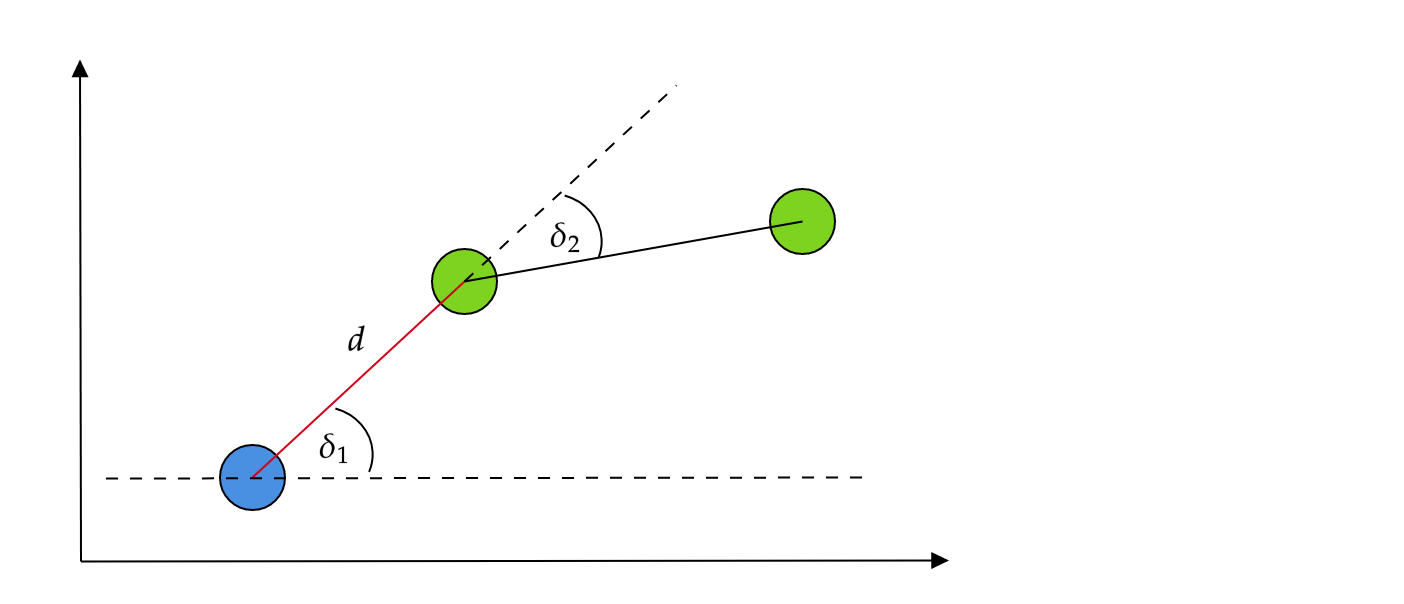
\includegraphics[width = 1.0\textwidth]{imgs/goal_sensor}
  \caption{Sensorik der Zielpeilung zwischen dem Fahrzeug (blau) und den nächsten beiden
  Wegpunkten (grün).   Dem Agent steht das Tupel $(d, \delta_1, \delta_2)$ bezüglich Zieldistanz,
  Trajektorie und Orientierung im Koordinatensystem zur Verfügung.}
  \label{fig:goal_sensor}
\end{figure}

Die Observation Spaces der Zielpeilung sind $[0, d_{max}]$, $[-\pi, \pi]$, wobei die maximal
mögliche Zielentfernung $d_{max} = \sqrt{(h_{map})^2 + (w_{map})^2}$ anhand der Ausmaße der
Karte bzgl. deren Breite $w_{map}$ und Höhe $h_{map}$ beschrieben wird. Der LiDAR-Sensor sendet
seine Strahlen gleichmäßig verteilt über den Öffnungswinkel $\varphi$ aus. Jeder Strahl wird
durch einen Observation Space von $[0, s_{max}]$ mit fester, maximaler Scanreichweite $s_{max}$
repräsentiert. Um die Route zielgerichteter fahren zu können, wird die Peilung des übernächsten
Ziels als Winkel zwischen der Fahrzeugposition und dem nächsten und übernächsten Zielpunkt
bereitgestellt, wie in Abbildung \ref{fig:goal_sensor} zu sehen ist. Dies entspricht
ebenfalls einem Observation Space von $[-\pi, \pi]$.\\

\begin{figure}[h]
  \centering
  
\includegraphics[width = 0.65\textwidth]{imgs/lidar_sensor}
  \caption{Schaubild eines LiDAR-Sensors mit Öffnungswinkel $\varphi$  und maximaler Scandistanz $s_{max}$.}
  \label{fig:linseg_circle_intersect}
\end{figure}

Da es unmöglich ist, die Bewegungsdynamiken der Fußgänger aus einem Standbild
erfasster Entfernungen durch den Strahlensensor abzuleiten, stehen dem Fahrzeug
immer mindestens die Strahlendaten der letzten 3 Zeitschritte zur Verfügung.

\subsection{Kartenmaterial: Statische und dynamische Entitäten}
Das Kartenmaterial setzt sich aus Vektorgrafiken zusammen, die die Fußgänger,
Hindernisse und das Fahrzeug repräsentieren. Hierbei werden Fußgänger und das
Fahrzeug als Kreise und Hindernisse als Liniensegmente in der 2D Ebene modelliert,
was der Umsetzung von PySocialForce entspricht.\\

Hindernisse haben eine statische Position und können verwendet werden,
um zusammengesetzte Entitäten wie Polygone oder aneinandergefügte Liniensegmente
zu repräsentieren. Fußgänger und Fahrzeuge sind hingegen dynamische Entitäten
und können sich auf der Karte bewegen.

\subsection{Kollisionserkennung}
Bei der Kollisionserkennung wird geprüft, ob das Fahrzeug mit anderen Entitäten
wie beispielsweise Fußgängern oder Hindernissen zusammengestoßen ist.
Dies entspricht einem Überlappen der geometrischen Formen, die die jeweiligen
Entitäten repräsentieren. Im Folgenden werden die dafür benötigten Formeln
hergeleitet und bezüglich effizienter Berechenbarkeit optimiert.

\subsubsection{Kollisionen zwischen Fahrzeug und Fußgängern}
Kollisionen zwischen dem Fahrzeug und Fußgängern können sehr einfach erkannt werden.
Als Distanzmetrik dient hierbei die euklidische Distanz zwischen den Kreiszentren
$C_{ped} = (x_{ped}, y_{ped})^T$ und $C_{veh} = (x_{veh}, y_{veh})^T$.
Ist die Distanz kleiner als die Summe der Kreisradien, schneiden sich die Kreise
und es liegt eine Kollision vor, wie in Abbildung \ref{fig:circle_intersect}
zu sehen ist. Die Konstellation in Fall 1, bei der sich ein Kreis vollständig innerhalb
des anderen Kreises befindet, wird ebenfalls als eine Kollision betrachtet.\\

\begin{figure}[h]
  \centering
  
\includegraphics[width = 1.0\textwidth]{imgs/circle_intersections}
  \caption{Fallbetrachtung möglicher Schnittpunkte zwischen zwei Kreisen mit Zentren $C_1$, $C_2$
  und Radien $r_1$, $r_2$. Nur in Fall 2 liegt keine Kollision vor.}
  \label{fig:circle_intersect}
\end{figure}

\begin{equation}
\begin{aligned}
dist(C_{ped}, C_{veh}) \le r_{ped} + r_{veh}
\end{aligned}
\end{equation}

\begin{equation}
\begin{aligned}
dist(C_{ped}, C_{veh}) = \lVert C_{veh} - C_{ped} \rVert
= \sqrt{(x_{ped} - x_{veh})^2 + (y_{ped} - y_{veh})^2}
\end{aligned}
\end{equation}

Um die kostspielige Quadratwurzelberechnung zu sparen, wird die Formel
auf beiden Seiten der Ungleichung quadriert. Die zusätzlich hinzugefügte Lösung
im negativen Wertebereich stellt kein Problem dar, da Distanzen und Kreisradien
immer $\ge 0$ sind. Somit ergibt sich:

\begin{equation}
\begin{aligned}
dist(C_{ped}, C_{veh})^2 \le (r_{ped} + r_{veh})^2
\end{aligned}
\end{equation}

\begin{equation}
\begin{aligned}
(x_{ped} - x_{veh})^2 + (y_{ped} - y_{veh})^2 \le (r_{ped} + r_{veh})^2
\end{aligned}
\end{equation}

Pro Zeitschritt muss für jeden der n Fußgänger geprüft werden, ob er mit dem Fahrzeug
kollidiert, was in linearer Zeit $O(n)$ mit $O(1)$ zusätzlichem Speicher durchgeführt
werden kann. Die damit verbundenen Operationen können zudem sehr effizient und
unabhänging voneinander berechnet werden.

\subsubsection{Kollisionen zwischen Fahrzeug und statischen Hindernissen}
Auch Kollisionen des Fahrzeugs mit Hindernissen müssen berechnet werden. Hierfür wird
die Menge aller auf dem Kreisbogen befindlichen Punkte mit der Menge aller auf
dem Liniensegment (Hindernis) befindlichen Punkten geschnitten, um alle potentiellen
Schnittpunkte zu bestimmen.\\

\begin{figure}[h]
  \centering
  
\includegraphics[width = 1.0\textwidth]{imgs/line_circle_intersections}
  \caption{Fallbetrachtung möglicher Schnittpunkte zwischen einem Liniensegment
  zwischen $P_1$, $P_2$ und einem Kreis mit Zentrum $C$ und Radius $r$.
  Nur in Fall 2 keine Kollision vor.}
  \label{fig:linseg_circle_intersect}
\end{figure}

Anhand der Kreisgleichung befindet sich ein Punkt $P$ genau dann auf der Kreislinie,
wenn die Distanz zwischen der Kreismitte $C$ und $P$ dem Radius $r$ des Kreises
entspricht. Vereinfachend wird die Kreismitte zum Ursprung verschoben, sodass
der Abstand zwischen Kreismitte und $P$ genau $\lVert P \rVert$ beträgt.

\begin{equation}
\begin{aligned}
M_{circle} = \{ P \epsilon R^2 | r = \lVert P \rVert \}
\end{aligned}
\end{equation}

Ein Hindernis ist als Liniensegment zwischen zwei Endpunkten $(P_1, P_2)$ definiert.
Die zugehörige Geradengleichung ergibt sich durch einen Punkt auf der Gerade plus
ein Vielfaches $\mu$ eines Richtungsvektors. In diesem Fall ist die Gerade durch
$P_1 - C$ und den Richtungsvektor $P_2 - P_1$ gegeben. Um ausschließlich auf
der Gerade befindliche Punkte innerhalb des Liniensegments zu erhalten, wird das
Vielfache $\mu$ des Richtungsvektors auf $0 \le \mu \le 1$ beschränkt.

\begin{equation}
\begin{aligned}
M_{line} = \{ \mu (P_2 - P_1) + (P_1 - C) | \mu \epsilon R \land 0 \le \mu \le 1 \}
\end{aligned}
\end{equation}

Nun kann die Schnittmenge der beiden Punktmengen $M_{line} \cap M_{circle}$
bestimmt werden, um auf Schnittpunkte bzw. Kollisionen zu prüfen. Hierfür wird
der von $P_1$ nach $P_2$ zeigende Vektor als $s = P_2 - P_1$ und der von
$C$ nach $P_1$ zeigende Vektor als $t = P_1 - C$ notiert.

\begin{equation}
\begin{aligned}
r = {\lVert \mu s + t \rVert} &\iff r^2 = {\lVert \mu s + t \rVert}^2\\
&\iff r^2 = (\mu s + t) \cdot (\mu s + t)\\
&\iff r^2 = \mu^2 s \cdot s + 2 \mu s \cdot t + t \cdot t\\
&\iff 0 = \mu^2 s \cdot s + 2 \mu s \cdot t + t \cdot t - r^2
\end{aligned}
\end{equation}

\begin{equation}
\begin{aligned}
a = s \cdot s, b = 2 s \cdot t, c = t \cdot t - r^2
\end{aligned}
\end{equation}

Dieses von $\mu$ abhängige Gleichungssystem führt zu einer quadratischen Gleichung
mit 0 bis 2 Lösungen, die durch die Lösungsformel für quadratische Gleichungen
bestimmt werden können.

\begin{equation}
\begin{aligned}
\mu_{1,2} = \frac{-b \pm \sqrt{D}}{2 a}, D = b^2 - 4 a c
\end{aligned}
\end{equation}

Das Gleichungssystem hat in den reellen Zahlen 0 Lösungen, wenn $D < 0$,
1 Lösung, wenn $D = 0$ und 2 Lösungen, wenn $D > 0$. Wie in Abbildung
\ref{fig:linseg_circle_intersect} dargestellt, liegt eine Kollision vor,
sofern $0 \le \mu \le 1$. Zudem besteht ein Sonderfall
einer Kollision, wenn sich das Liniensegment vollständig innerhalb des Kreises
befindet, was gesondert geprüft werden muss. Da jede Prüfung in konstanter Zeit
möglich ist, ergibt sich für $o$ Hindernisse eine Zeitkomplexität von $0(o)$;
die Speicherkomplexität ist konstant.

\subsection{Simulation radialer Strahlensensoren (LiDAR)}
Ein radialer Strahlensensor sendet eine gewisse Anzahl an Strahlen aus, deren
Ausrichtungen gleichmäßig über den Öffnungsbereich des Sensors verteilt sind.
Für jeden Strahl muss die Distanz zwischen der Strahlenquelle und der
nächstgelegenen, getroffenen Entität innerhalb des Suchradius berechnet werden.
Es ergibt sich demnach für $r$ Strahlen, $p$ Fußgänger und $o$ Hindernisse eine
Zeitkomplexität von $O({r (p + o)})$ und eine Speicherkomplexität von $O(r)$.

\subsubsection{Entfernungen zu Fußgängern}
Um die Entfernung zwischen einer Strahlenquelle und einem vom Strahl getroffenen
Fußgänger zu berechnen, wird der Fußgänger als Kreis und der Strahl als eine von
der Strahlenquelle ausgehende Halbgerade modelliert. Die Richtung des Strahls
ist durch den Einheitsvektor $v_{ray}$ gegeben.\\

Die Formel zur Kollisionsberechnung zwischen einer Linie und einem Kreis wurde
bereits für Kollisionen zwischen Fahrzeugen und Hindernissen hergeleitet. Im Gegensatz
zum vorherigen Anwendungsfall ist aber nicht nur relevant, ob eine Kollision vorliegt,
sondern auch wie weit sie entfernt ist.
Hierfür werden ebenfalls $\mu_{1,2}$ bestimmt und anschließend in die Formel $P_{Gerade}$
eingesetzt, um die beiden Schnittpunkte $S_1, S_2$ zu bestimmen. Falls es
keine Schnittpunkte gibt, ist die Entfernung $\infty$. Bei exakt einem Schnittpunkt
ist $S_1 = S_2$, was o.B.d.A. nicht weiter betrachtet werden muss.\\

Nun kann die kürzeste Entfernung von der Strahlenquelle zu den Schnittpunkten
$S_1, S_2$ als  $min(dist(P_{sensor}, S_1), dist(P_{sensor}, S_2))$ bestimmt werden.
Allerdings ist hierbei zu beachten, dass der Vektor von der Strahlenquelle zum
Schnittpunkt ein positives Vielfaches des Strahlenvektors $v_{ray}$ sein muss,
da sich der Strahl nur in diese Richtung ausbreitet. Dies kann durch $\mu \ge 0$
geprüft werden.

\begin{equation}
\begin{aligned}
\mu_{1,2} = \frac{-b \pm \sqrt{D}}{2 a}, D = b^2 - 4 a c\\
a = s \cdot s, b = 2 s \cdot t, c = t \cdot t - r^2
\end{aligned}
\end{equation}

Um sich im Fall, dass keine Kollision vorliegt, die Quadratwurzelberechnung
$\sqrt{D}$ zu sparen, wird nochmals die Lösungsformel für quadratische Gleichungen
betrachtet. Da $a = \lVert s \rVert^2 \implies 2a > 0$, gibt es genau dann keine Kollision,
wenn entweder $D < 0$ oder $-b \pm \sqrt{D} < 0$.

\begin{equation}
\begin{aligned}
-b \pm \sqrt{D} < 0 \iff -b + \sqrt{D} < 0 \iff \sqrt{D} < b \iff b > 0 \land b^2 > D
\end{aligned}
\end{equation}

Somit kann die Prüfung auf $\mu < 0$ durch $b > 0$ und $b^2 > D$ ersetzt werden.

\subsubsection{Entfernungen zu Hindernissen}
Zur Entfernungsberechnung zwischen einer Strahlenquelle und Hindernissen wird
eine neue Berechnungsformel benötigt, die eine Halbgerade (Strahl) mit einen
Liniensegment (Hindernis) schneidet.
Die Halbgerade ist gegeben durch die Position der Strahlenquelle $P_{sensor}$ und
den Richtungsvektor $v_{ray}$ des Strahls als Einheitsvektor; das Liniensegment zwischen
$P_1$ und $P_2$ ist durch den Punkt $P_1$ und den Richtungsvektor $v_{seg} = P_2 - P_1$
definiert. Bei der Halbgerade sind nur Vielfache $\tau \ge 0$ des Richtungsvektors
erlaubt, beim Liniensegment nur Vielfache $\mu \in [0, 1]$.\\

\begin{figure}[h]
  \centering
  
\includegraphics[width = 1.0\textwidth]{imgs/lineseg_intersections}
  \caption{Fallbetrachtung möglicher Schnittpunkte zwischen zwei Liniensegmenten,
  jeweils definiert durch ihre Endpunkte $P_1$, $P_2$ bzw. $P_3$, $P_4$.
  Parallele Linien wie in Fall 3 schneiden sich nicht. Außerdem sind die
  Enden der Segmente zu beachten.}
  \label{fig:linseg_intersect}
\end{figure}

Nun können die beiden Punktmengen $M_{ray}$ und $M_{obstacle}$ aufgestellt und deren
Schnittmenge $M_{ray} \cap M_{obstacle}$ bestimmt werden, um alle Schnittpunkte zu erhalten.

\begin{equation}
\begin{aligned}
M_{ray} = \{ P_{sensor} + \tau v_{ray} | \tau \in R, \tau > 0 \}
\end{aligned}
\end{equation}

\begin{equation}
\begin{aligned}
M_{obstacle} = \{ P_1 + \mu v_{seg} | \mu \in R, 0 \le \mu \le 1 \}
\end{aligned}
\end{equation}

\begin{equation}
\begin{aligned}
M_{ray} \cap M_{obstacle} =
\{ P_1 + \mu v_{seg} | \mu \in R, P_{sensor} + \tau v_{ray} = P_1 + \mu v_{seg} \}
\end{aligned}
\end{equation}

Dies ergibt ein von den Unbekannten $\tau$ und $\mu$ abhängiges Gleichungssystem,
bestehend aus zwei Gleichungen bezüglich der linear unabhängigen x/y Koordinaten
der Vektoren. Das Gleichungssystem ist also eindeutig lösbar.

\begin{equation}
\begin{aligned}
&P_{sensor} = (x_{sensor}, y_{sensor})^T, P_1 = (x_1, y_1)^T,\\
&v_{ray} = (x_{ray}, y_{ray})^T, v_{seg} = (x_{seg}, y_{seg})^T\\
&v_{diff} = (x_{diff}, y_{diff})^T = P_1 - P_{sensor}
\end{aligned}
\end{equation}

\begin{equation}
\begin{aligned}
I)& \, x_{sensor} + \tau x_{ray} = x_1 + \mu x_{seg}\\
II)& \, y_{sensor} + \tau y_{ray} = y_1 + \mu y_{seg}
\end{aligned}
\end{equation}

Durch Umformen ergeben sich folgende nach $\tau$ aufgelöste Gleichungen:

\begin{equation}
\begin{aligned}
I')& \, \tau = \frac{\mu x_{seg} + x_{diff}}{x_{ray}}\\
II')& \, \tau = \frac{\mu y_{seg} + y_{diff}}{y_{ray}}
\end{aligned}
\end{equation}

Nun wird $\tau$ durch Gleichsetzen eliminiert. Anschließend wird nach $\mu$ aufgelöst,
um die Lösung des Gleichungssystems zu bestimmen.

\begin{equation}
\begin{aligned}
\frac{\mu x_{seg} + x_{diff}}{x_{ray}} = \frac{\mu y_{seg} + y_{diff}}{y_{ray}}
\end{aligned}
\end{equation}

\begin{equation}
\begin{aligned}
\mu \frac{x_{seg}}{x_{ray}} + \frac{x_{diff}}{x_{ray}}
= \mu \frac{y_{seg}}{y_{ray}} + \frac{y_{diff}}{y_{ray}}
\end{aligned}
\end{equation}

\begin{equation}
\begin{aligned}
\mu \frac{x_{seg}}{x_{ray}} - \mu \frac{y_{seg}}{y_{ray}}
= \frac{y_{diff}}{y_{ray}} - \frac{x_{diff}}{x_{ray}}
\end{aligned}
\end{equation}

\begin{equation}
\begin{aligned}
\mu \left(\frac{x_{seg} y_{ray}}{x_{ray} y_{ray}} - \frac{x_{ray} y_{seg}}{x_{ray} y_{ray}}\right)
= \frac{x_{ray} y_{diff}}{x_{ray} y_{ray}} - \frac{y_{ray} x_{diff}}{x_{ray} y_{ray}}
\end{aligned}
\end{equation}

\begin{equation}
\begin{aligned}
\mu \frac{x_{seg} y_{ray} - x_{ray} y_{seg}}{x_{ray} y_{ray}}
= \frac{x_{ray} y_{diff} - y_{ray} x_{diff}}{x_{ray} y_{ray}}
\end{aligned}
\end{equation}

\begin{equation}
\begin{aligned}
\mu (x_{seg} y_{ray} - x_{ray} y_{seg}) = x_{ray} y_{diff} - y_{ray} x_{diff}
\end{aligned}
\end{equation}

\begin{equation}
\begin{aligned}
\mu = \frac{x_{ray} y_{diff} - y_{ray} x_{diff}}{x_{seg} y_{ray} - x_{ray} y_{seg}},
x_{seg} y_{ray} - x_{ray} y_{seg} \neq 0
\end{aligned}
\end{equation}

Wenn $x_{seg} y_{ray} - x_{ray} y_{seg} \neq 0$, ergibt sich der Schittpunkt
$S = P_1 + \mu v_{seg}$ durch Einsetzen von $\mu$ in $M_{obstacle}$.
$\tau$ kann über $\tau = \frac{\mu x_{seg} + x_{diff}}{x_{ray}}$ oder
$\tau = \frac{\mu y_{seg} + y_{diff}}{y_{ray}}$ bestimmt werden.
Nun muss noch überprüft werden, ob $0 \le \mu \le 1$ und $\tau \ge 0$. Ist dies der Fall,
trifft der Strahl das Hindernis nach einer Entfernung von $dist(P_{sensor}, S)$,
andernfalls ist die Distanz $\infty$.
Wenn $x_{seg} y_{ray} - x_{ray} y_{seg} = 0$, steht der Strahl parallel zum Hindernis
und verfehlt, da Hindernisse keine Tiefe besitzen.

\subsubsection{Nachbereitung der berechneten Entfernungen}
Nachdem die Kollisionsberechnungen für alle Strahlen und Entitäten durchgeführt wurden,
kann die minimale Entfernung $d_{ray}$ pro Strahl bestimmt werden.
Entfernungen, die noch auf $\infty$ initialisiert sind, da keine Kollision vorliegt,
werden mit $d_{ray} = min(d_{ray}, s_{max})$ auf die maximale Scanreichweite
des Sensors beschränkt.\\

Nun wird zur bisher perfekten Messung ein leichtes Rauschen hinzugefügt, was vor allem
für das Training einer Künstlichen Intelligenz wichtig ist, um Overfitting vorzubeugen.
Hierbei gehen Strahlen mit einer gewissen Wahrscheinlichkeit $P_{lost}$ ganz verloren,
sodass die gemessene Distanz der maximalen Scanreichweite entspricht.
Zudem können auch Messungen mit der Wahrscheinlichkeit $P_{corrupt}$ verfälscht werden,
sodass die Entfernung zufällig um einen gleichverteilten Faktor $f \in [0, 1]$
skaliert wird. Empfohlene Wahrscheinlichkeiten sind $P_{lost} = 0.005$
und $P_{corrupt} = 0.002$.

\subsection{Steuerung der Fußgänger}
Bezüglich der Simulation von realistischem Fußgängerverhalten, wird das Social Force Modell
aus Abschnitt \ref{sec:SocialForce} verwendet, um Fußgänger einzeln oder in Gruppen zu einem
Zielort zu bewegen.
Eine Gruppe ist am Ziel, wenn sich ihr Massenschwerpunkt $\frac{1}{n} \sum_{i=1}^n p_i$
zu einem diskreten Zeitpunkt $t$ nah genug am Zielpunkt befindet. O.B.d.A. sind einzelne
Fußgänger als eine Gruppe mit nur einem Fußgänger definiert. Da Fußgängerzonen und Gehwege
simuliert werden sollen, wird im Folgenden betrachtet, wie ein entsprechendes Verhalten
erzielbar ist.\\

Zur Simulation von Fußgängerzonen werden zunächst Zonen definiert, in denen sich
die Fußgänger aufhalten. Um ein Verhalten zu erzielen, bei dem die Fußgänger
durcheinander laufen, werden gleichverteilt zufällige Zielpunkte innerhalb
der Zone gewählt, zu denen die Fußgänger laufen. Sobald ein Ziel erreicht ist,
wird ein neues, zufälliges Ziel bestimmt.
Das stationäre Verhalten in Fußgängerzonen wird durch das zielgerichtete Laufen
von Routen ergänzt, was eher dem Fußgängerverhalten auf Gehwegen entspricht.
Ähnlich wie bei der Globalen Navigation des Fahrzeugs werden die Routen zwischen Start-
und Zielzone anhand von groben Wegpunkten vorgegeben. Sobald ein Wegpunkt erreicht ist,
wird der nächste angesteuert. Sind die Fußgänger am finalen Ziel innerhalb der
Zielzone, erscheinen sie wieder in der Startzone, um die Route erneut zu laufen.\\

Entsprechend der vorgegebenen Fußgängerdichte, d.h. Fußgänger pro Fläche, werden allen Routen
und Fußgängerzonen eine Anzahl an Fußgängern gemäß ihrer Fläche zugewiesen. Die Gehwegfläche
wird durch die Multiplikation der jeweiligen Routenlänge mit einer angenommenen Gehwegbreite
von 3-4 Metern geschätzt. Wie in Moussaïd et. al \cite{moussaid2010groupssf} beschrieben ist
die Größe der Gruppen poissonverteilt. Daher wird vor der Zuteilung der Fußgänger zunächst
die Anzahl der Gruppenmitglieder gemäß der Wahrscheinlichkeitsverteilung gezogen.
Anschließend werden die Massenschwerpunkte der Gruppen gleichverteilt innerhalb der
Fußgängerzonen bzw. entlang der Routen bestimmt und deren Gruppenmitglieder normalverteilt
um den Schwerpunkt positioniert.


\section{Technische Umsetzung der Simulationsumgebung}
Zum Erlernen autonomer Fahrverhaltensweisen wird ein Simulator anhand der Beschreibung
aus Abschnitt \ref{sec:SimEnv} in Python umgesetzt. Das sehr ähnliche Projekt \emph{RobotSF}
der Universität Triest von Caruso et. al \cite{machines11020268} wird hierfür als Basis verwendet
und entsprechend adaptiert. In der ursprünglichen Version von \emph{RobotSF} steht sowohl
ein steuerbares Fahrzeug mit entsprechender Sensorik und Aktuatorik, als auch die
Simulation der Fußgänger mittels Social Force durch das Paket \emph{PySocialForce}
\cite{gao2020pysf} bereit. Die Implementierung des Simulators bezüglich der Differential
Drive Kinematik, des LiDAR-Sensors, der Fußgängersteuerung und der Kollisionslogik ist
von Caruso et. al und wird entsprechend der Konzeption aus Abschnitt \ref{sec:SimEnv} angepasst.
Die Schnittstelle der Simulationsumgebung zur Umsetzung der Trainingsalgorithmen von
Caruso et. al wird zugunsten einer breiteren Kompatibilität mit Implementierungen gängiger
Trainingsalgorithmen wie beispielsweise \emph{Stable Baselines 3} \cite{raffin2021sb3}
zu einer \emph{OpenAI Gym} Schnittstelle \cite{brockman2016openai} umgestellt. Da es sich
bei der Umsetzung der Simulationsumgebung um eine Erweiterung handelt, wird diese
im Folgenden \emph{RobotSF} genannt.

\subsection{Visualisierung der Simulationsumgebung}
Da die ursprüngliche Simulationsumgebung über keine Live-Visualisierung verfügt,
wird eine entsprechende Komponente zu \emph{RobotSF} hinzugefügt, wie in Abbildung
\ref{fig:SimPyGame} zu sehen ist. Die Ansicht verwendet die Visualisierungstechnologie
\emph{PyGame}, womit eine ausreichende Performanz für die flüssige Darstellung von
Bewegungen erzielt werden kann. Vergleichbare Technologien wie \emph{Tkinter} oder
\emph{Turtle} sind zu langsam und kommen daher nicht in Betracht.\\

\begin{figure}[h]
  \centering
  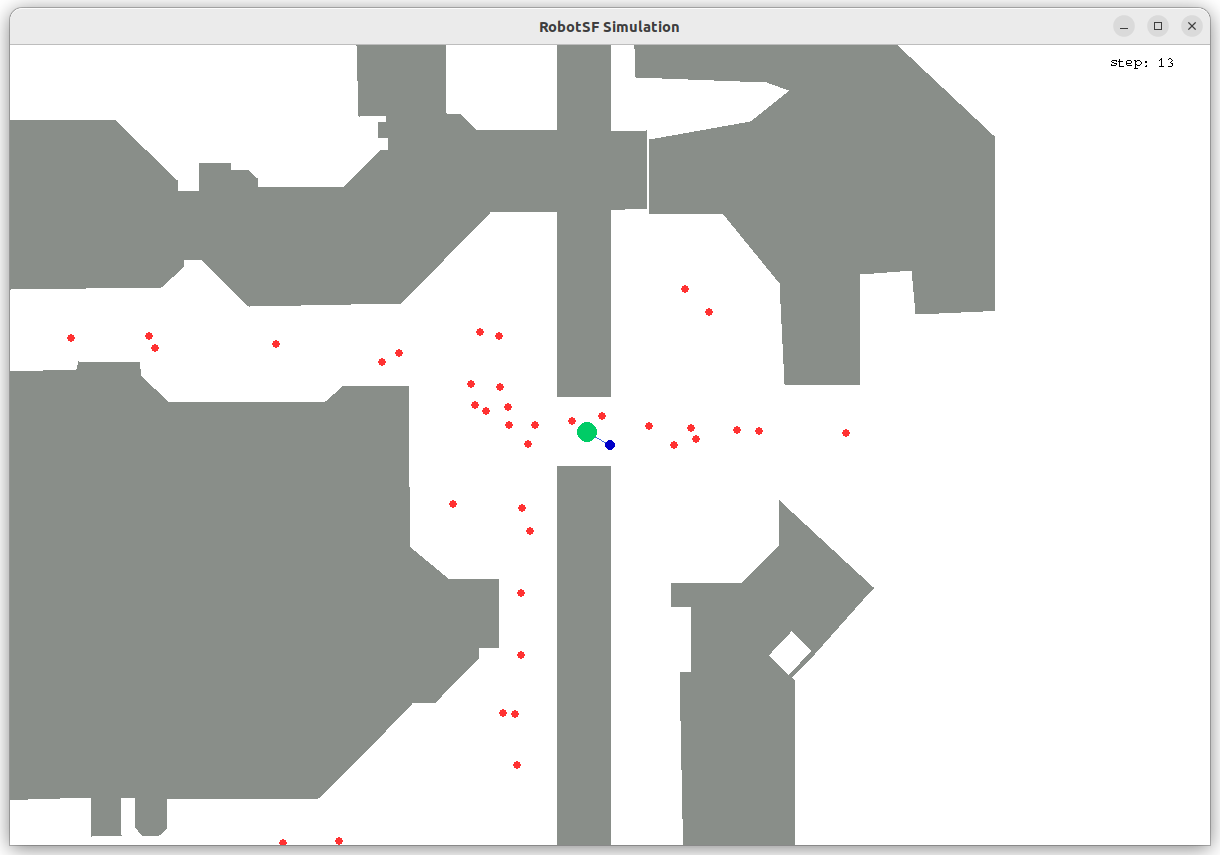
\includegraphics[width = 0.65\textwidth]{imgs/simulator_reworked}
  \caption{Simulatoranzeige mit PyGame}
  \label{fig:SimPyGame}
\end{figure}

Die dargestellten Entitäten umfassen das Fahrzeug (blauer Kreis), Fußgänger (rote Kreise)
und Hindernisse (graue Polygone). Zudem werden die Zielzonen der anzusteuernden
Wegpunkte (grüne Kreise) und der Dynamikvektor des Fahrzeugs (blaue Linie)
augmentiert. Die Kamera blickt senkrecht von oben auf die simulierte 2D-Ebene
und zentriert das betrachtete Fahrzeug in der Mitte des Bildschirms. Zudem kann
auch der Zoom-Faktor zu Beginn der Simulation passend eingestellt werden.\\

\subsection{Aufbereitung des Kartenmaterials}
Zur Bearbeitung des Kartenmaterials wird das Werkzeug \emph{Map Editor} entwickelt.
Wie in Abbildung \ref{fig:MapEditor} zu sehen ist, besteht der \emph{Map Editor} aus einem
Texteditor auf der linke Seite und einer Live-Vorschau der Karte auf der rechte Seite,
sodass mit vertretbarem Aufwand neue Trainingsszenarien erstellt werden können. Durch ein
weiteres Skript können Gebäudeumrisse maßstabsgetreu aus OpenStreetMap geladen werden,
was das Importieren von echtem Kartenmaterial auf einfache Weise ermöglicht. Per Linksklick
in die Vorschauanzeige werden die Koordinaten an der entsprechenden Stelle auf der Karte
ausgegeben, sodass sich Zonen und Routen leicht einpflegen lassen.\\

\begin{figure}[h]
  \centering
  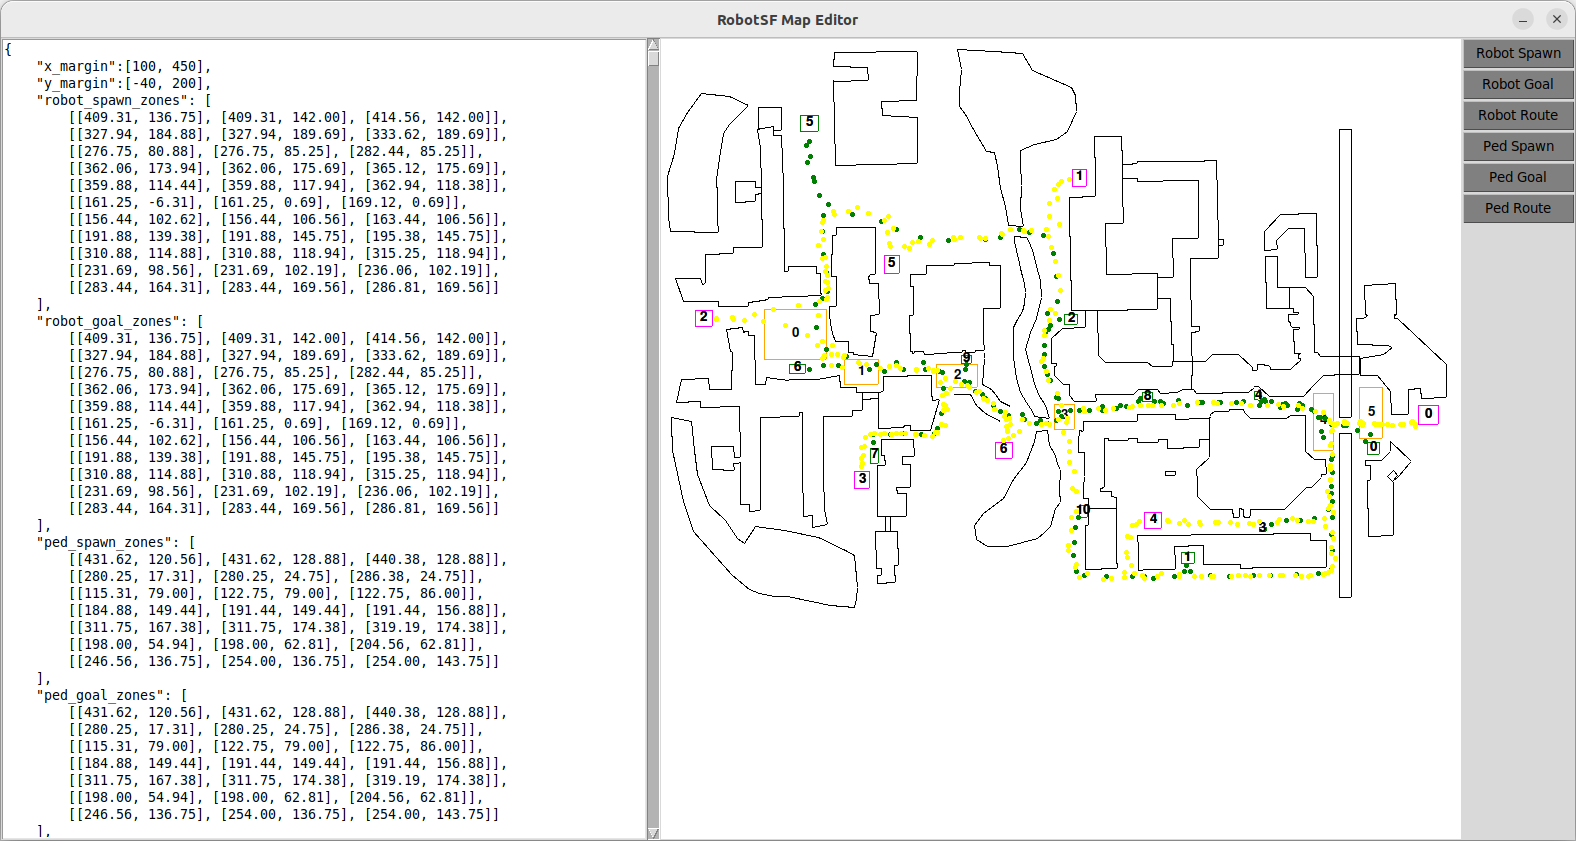
\includegraphics[width = 1.0\textwidth]{imgs/map_editor}
  \caption{Map Editor mit Texteingabe auf der linken und Vorschau auf der rechten Seite.
           Die Vorschau zeigt den Campus der Universität Augsburg. Im Text Editor
           wird das Kartenmaterial bearbeitet.}
  \label{fig:MapEditor}
\end{figure}

Für den Map Editor wird Tkinter als Visualisierungstechnologie gewählt,
da PyGame über keine vorgefertigten Bausteine zur Texteingabe verfügt und somit
ausscheidet. Zudem erfordert die Vorschau des Kartenmaterials ohnehin keine hohen
Bildraten für eine flüssige Darstellung, sodass stattdessen auf die Canvas-Funktion
von Tkinter zurückgegriffen wird. Ein vollkommen visuelles Bedienkonzept ohne
die Notwendigkeit einer manuellen Bearbeitung des Kartenmaterials im Texteditor stellt
eine Alternative dar, wird jedoch aufgrund des niedrigen Mehrwerts bei gleichzeitigem,
erheblichem Mehraufwand für das Projekt verworfen.
Es wäre vorgesehen gewesen, die einzelnen Zonen, Wegpunkte und Hindernisse per Mausklick
einzufügen. Per Schaltfläche wählt der Bearbeiter die einzufügende Struktur aus.
Anschließend setzt er die Umrisse per Linksklick in die Kartenvorschau. Ein Rechtsklick
bricht das Einfügen ab. Ist keine Schaltfläche aktiv, werden die Entitäten beim Bewegen
des Mauszeigers über ihre unmittelbare Umgebung hervorgehoben. Wird während der
Hervorhebung zusätzlich ein Recktsklick ausgeführt, löscht dies die Entität. Das Setzen
der Kartenumrisse löscht immer die vorherigen Umrisse. Per Drehung des Mausrads
kann wie gewöhnlich gezoomt werden.\\


\subsection{Konzeption der Trainingsumgebung} \label{sec:TrainingApproach}
Der \emph{RobotSF} Simulator des Forscherteams aus Triest sieht bereits vor,
zufallsgeneriertes Kartenmaterial mit Hindernissen (Polygone) zu erzeugen und
als JSON-Dateien zu speichern. Wie in Abbildung \ref{fig:MapOld} zu sehen ist, besteht
das Kartenmaterial aus unregelmäßigen, sternförmigen Hindernissen, was mehr einer
Mondlandschaft anstatt einem Gehweg oder einer Fußgänerzone entspricht. Die unrealistischen
Formen von \emph{RobotSF} werden daher durch echtes, aus OpenStreetMap importiertes
Kartenmaterial ersetzt und mithilfe des \emph{Map Editors} aufbereitet. Dies erfordert
eine Effizienzoptimierung der Simulationsumgebung, auf die im darauffolgenden Abschnitt
\ref{sec:SimEffOpt} eingegangen wird.

\begin{figure}[h]
  \centering
  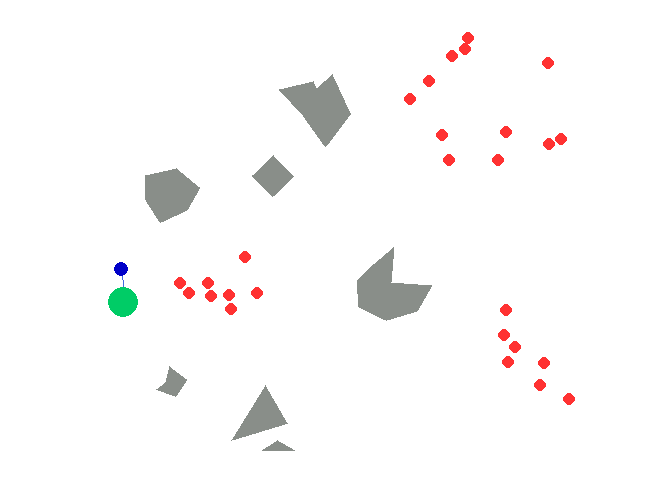
\includegraphics[width = 0.65\textwidth]{imgs/kartenmaterial_alt}
  \caption{Beispiel für altes Kartenmaterial des \emph{RobotSF} Simulators}
  \label{fig:MapOld}
\end{figure}

Als Kartenmaterial für die Trainingsumgebungen werden zwei echte Karten gewählt. Wie in
Abbildung \ref{fig:Scenario_1} zu sehen ist, besteht die erste Trainingsumgebung aus
einigen miteinander verbundenen Häuserblocks nahe des Universitätsgeländes, in deren
Innenhöfen künstliche, in orange dargestellte Fußgängerzonen angelegt werden, um belebte
Plätze zu simulieren. Das Fahrzeug startet in der blau markierten Zone und folgt den
durch die grünen Punkte dargestellten Routen bis hin zur jeweiligen Zielzone. Die Routen
verlaufen in alle Himmelsrichtungen und führen bewusst durch mindestens eine Menschenmenge.\\

\begin{figure}[h]
  \centering
  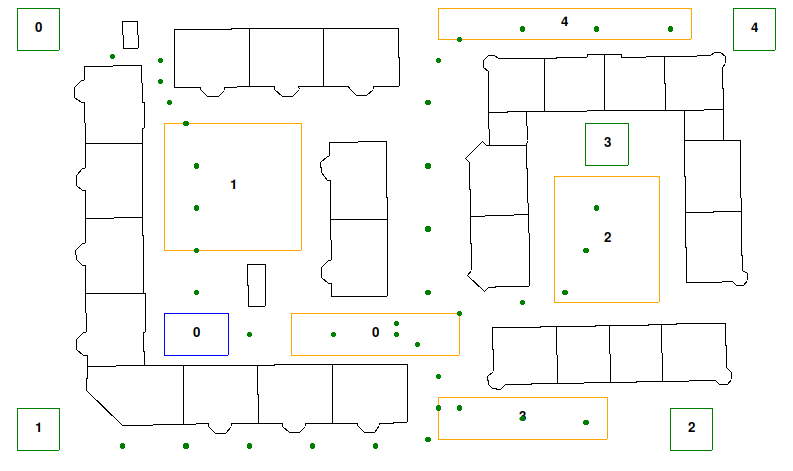
\includegraphics[width = 1.0\textwidth]{imgs/small_map}
  \caption{Erste Trainingsumgebung des überarbeiteten \emph{RobotSF} Simulators}
  \label{fig:Scenario_1}
\end{figure}

Dadurch dass der Agent gezwungen wird, durch Menschenmengen zu fahren, soll die sichere
Interaktion mit Fußgängern erlernt werden. Die Verkehrsdichte in den orange markierten
Fußgängerzonen kann während der Trainingsläufe und Evaluationen variiert werden, um die
Robustheit der erlernten Fahrverhaltensweise zu prüfen. Durch das Ein- und Ausschalten
der \emph{Ped-Robot Force} wird das Verhalten der Fußgänger dahingehend modifiziert,
ob sie das Fahrzeug wahrnehmen können und ihm ausweichen. Durch die Modifikation des
Fußgängerverhaltens bezüglich der Wahrnehmung des Fahrzeugs während des Trainings soll
gesteuert werden, ob der Agent offensiveres oder defensiveres Fahrverhalten lernt.\\

Für die zweite Trainingsumgebung wird eine Karte des Campus der Universität Augsburg
gewählt, da sich entsprechendes Kartenmaterial als verkehrsberuhigter Bereich mit viel
Fußgängerverkehr bestens für die virtuelle Erprobung autonomer Mikromobilitätsahrzeuge
anbietet und auch perspektivisch die Evaluationen echter Fahrzeuge in der Realität ermöglicht.
Wie in Abbildung \ref{fig:Scenario_2} zu sehen, umfassen die in grün dargestellten Start- und
Zielorte des Fahrzeugs das Unikum (0), das Rote Pferd (1), die Alte Cafeteria (2),
den Durchgang zwischen N-Gebäude und Mensa (3), das Prüfungsamt (4), den Ausgang zum
Messeparkplatz (5), die Juristische Fakultät (6), den Eingang zur Wirtschaftsinformatik (7),
den Eingang zum C-Hörsaal (8), den Eingang zur Zentralbibliothek (9) und den Eingang zur
mathematisch-naturwissenschaftlichen Bibliothek (10).
Am Wasserspiel (0, 1), vor der Zentralbibliothek (2), vor der Brücke (3) und bei den
Straßenbahnhaltestellen (4, 5) befinden sich die orange markierten Fußgängerzonen, um dichten
Verkehr zu simulieren. Zudem verlaufen auf allen befahrenen Gehwegen die mit gelben Punkten
dargestellten Fußgängerrouten in beide Laufrichtungen, um typischen Verkehr zu generieren.\\

\begin{figure}[h]
  \centering
  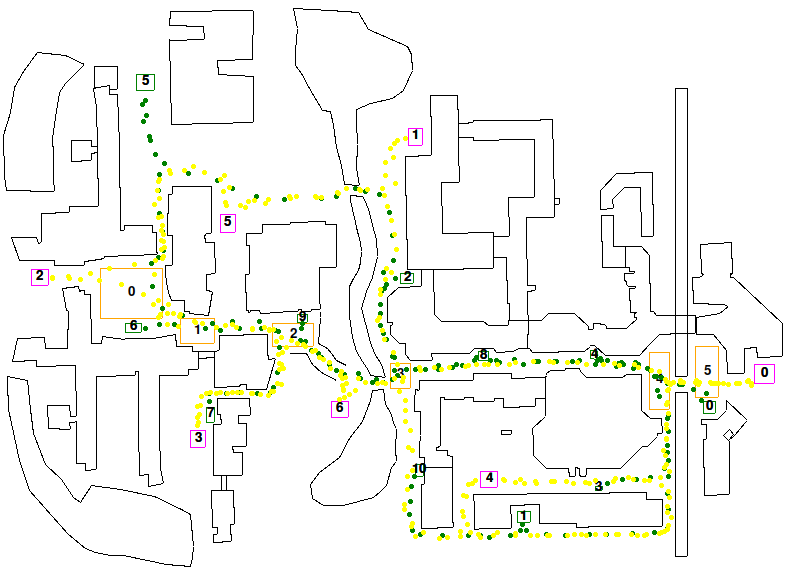
\includegraphics[width = 1.0\textwidth]{imgs/campus_map}
  \caption{Zweite Trainingsumgebung des überarbeiteten \emph{RobotSF} Simulators.
  Das Kartenmaterial zeigt den Campus der Universität Augsburg.}
  \label{fig:Scenario_2}
\end{figure}

Das Design der Routen sieht vor, verschiedenste Situationen herbeizuführen, die auch
in der Realität auftreten können. Auf den Gehwegen wird hauptsächlich getestet,
ob der Agent die Bewegung der Fußgänger korrekt einschätzen und Überholmanöver
in engen Räumen sicher durchführen kann. Nah an Hauswänden verlaufende 90-Grad Kurven
prüfen, ob vor der Kurve abgebremst wird, da der Agent nur eine eingeschränkte Sicht
auf den sich hinter der Wand befindlichen Gegenverkehr hat. Hingegen wird auf großen,
belebten Plätzen wie bereits bei der ersten Trainingsumgebung die Fähigkeit zur
Kollisionsvermeidung und Erzielung von Fortschritten in dichten Menschenmengen getestet.
Dabei soll der Agent ein möglichst defensives Verhalten aufweisen, damit sich die Fußgänger
sicher fühlen können. Durch Engstellen soll der Agent lernen, erst zu fahren, sobald eine
befahrbare Passage frei wird. Dies erfordert unter anderem eine Einschätzung, ob die
Engstelle lange genug befahrbar bleibt, um sie zu passieren.


\section{Effizienzoptimierung der Simulationsumgebung} \label{sec:SimEffOpt}
Nach einem Austausch mit dem Forscherteam hinter \emph{RobotSF} wird klar, dass ein
effizientes Training von Fahragenten an erheblichen Effizienzproblemen der
Simulationsumgebung leidet. Die Forscher geben Trainingszeiten von bis zu einem Monat an.
Aufgrund des beschränkten zeitlichen Rahmens dieser Arbeit sind entsprechende Wartezeiten
nicht hinnehmbar, weshalb die Umsetzung durch effizientere Algorithmen und Datenstrukturen
optimiert wird. Zur Messung der Effizienz dient ein Skript, das 10000 Simulationsschritte
ausführt und dabei zufällige Aktionen auswählt. Mithilfe von Scalene
\cite{berger2022triangulating} kann der Beitrag jeder Zeile aus dem Python Quellcode
gemessen werden, um kritische Komponenten zu identifizieren. Anhand der Performance-Profile
ist ersichtlich, dass hauptsächlich der Kraftberechnung von PySocialForce und die
von Caruso et. al umgesetzten Komponenten des LiDAR-Sensors und der Kollisionserkennung
zur Rechenzeit beitragen. Alle restlichen Zeiten werden unter dem Punkt
\glqq{}Sonstige\grqq{} zusammengefasst, wie in Tabelle \ref{tab:SimEffOpt} dargestellt.\\

\begin{table}
\centering
\begin{tabular}{ |p{4cm}||c|c|c|c|c|c| }
 \hline
 Performance-Profil vs. Simulatorversion & Total & PySF & Koll. & LiDAR & Sonst. & Speedup \\
 \hline \hline
 Unoptimized          & 289s & 36\% & 34\% & 19\% & 11\% &  - \\ \hline
 Fast Grid Raycast    & 132s & 76\% & 13\% &  5\% &  6\% & 2.26x \\ \hline
 Fast Grid Map        &  82s & 78\% &  2\% &  9\% & 11\% & 1.61x \\ \hline
 Fast Obstacle Force  &  61s & 74\% &  3\% & 12\% & 11\% & 1.34x \\ \hline
 Continuous Map Algos &  59s & 72\% & 10\% &  6\% & 12\% & 1.03x \\ \hline
 No Custom Forces     &  15s & 30\% &  5\% & 15\% & 50\% & 3.93x \\ \hline
\end{tabular}
\caption{Performance-Profile der jeweiligen Simulatorversionen. Es sind die Gesamtrechenzeit
in Sekunden und die jeweiligen Anteile der Komponenten an der Gesamtzeit in Prozent zu sehen.
Die Spalte \glqq{}Speedup\grqq{} zeigt den jeweiligen Faktor der erzielten Beschleunigung
zur vorherigen Simulatorversion.}
\label{tab:SimEffOpt}
\end{table}

Anhand des ersten Profils entfallen ca. 48\% auf eine Datei namens \glqq{}map.py\grqq{},
die sowohl die Logik zur Kollisionserkennung, als auch die Umsetzung des LiDAR-Sensors
enthält. Daher wird die Repräsentation des Kartenmaterials nun genauer betrachtet. Es stellt
sich heraus, dass die Karte durch eine Rasterstruktur (2D-Bitmaske) umgesetzt wird, wobei
ein Bit pro Zelle angibt, ob sich dort Hindernisse befinden. Zum Aufbau des Rasters werden
die Umrisse aller Entitäten berechnet und anschließend per bitweisem OR zu einer Maske
(engl. Occupancy Grid) zusammengefügt. Umrisse statischer Entitäten werden zu Beginn der
Simulation vorberechet und um die dynamisch berechneten Umrisse aller beweglichen
Entitäten zu jedem Simulationsschritt ergänzt.\\

Vorteile der Datenstruktur bestehen zunächst darin, dass die Komplexität der Algorithmen,
die auf einem fertig berechneten Raster arbeiten, lediglich mit der Rastergröße skaliert,
nicht aber mit der Anzahl der dargestellten Objekte. Die Kollisionsberechnung des
Fahrzeugs kann beispielsweise mittels bitweisem AND der Fahrzeugumrisse mit den
Hindernissen auf der Karte umgesetzt werden. Der Vorteil der Skalierbarkeit ist jedoch
ein Trugschluss, da die Anzahl an simulierten Objekten für einen tatsächlichen Vorteil
größer als die Anzahl der Rasterzellen sein muss. Weitere Nachteile ergeben sich, da das
Sichtfeld des Fahrzeugs mit $O(r^2 d^2)$ bzgl. des Sichtradius $r$ und der Rasterdichte
$d$ skaliert und somit dem \glqq{}Curse of Dimensionality\grqq{} unterliegt, der sich
zudem verstärkt, falls eine feingranularere Rasterisierung der Karte benötigt wird.
Für \emph{RobotSF} wird beispielsweise ein quadratisches Raster mit einer Seitenlänge
von 40 Metern gewählt, dessen Zellen eine Seitenlänge von 0.1 Meter aufwiesen.
Dies entspricht einem Vielfachen von 160000 Rechenzyklen pro Rasteroperation.
Abgesehen von einem erheblichen Verlust an Genauigkeit sind Algorithmen mit Bitmasken
auch sehr ineffizient, da die restlichen Programmteile von \emph{RobotSF} ohnehin mit
Vektorgrafiken arbeiten und daher zu jedem Zeitschritt die Konvertierung aller beweglichen
Objekte in Bitmasken erfordern.
Auch die Umsetzung eines LiDAR-Sensors bzgl. einer Rasterstruktur ist eher umständlich,
da die Strahlen als Pixelgeraden, z.B. mit Bresenham's Line \cite{bresenham65linealgo},
berechnet werden müssen, um dann einen Abgleich der Bitmasken durchführen zu können.
Um die Kompatibilität zur alten Grid-Struktur von Caruso et. al beibehalten zu können, wird
zunächst der LiDAR-Sensor und anschließend die Kollisionserkennung mit Numba optimiert,
indem die Algorithmen dahingehend verbessert werden, möglichst viele Befehle in generierten
C Code auszulagern. Dies führt zu ersten Erfolgen, sodass die Rechenzeiten von vormals 158
Sekunden auf 9 Sekunden gesenkt werden können, was im Bezug auf die Gesamtrechenzeit eine
3.6-fache Beschleunigung erlaubt.\\

Nun stellen die Kraftberechnungen von PySocialForce mit 78\% den Hauptanteil am Profil,
sodass diese im Folgenden näher betrachtet werden. Um den kritischen Pfad von PySocialForce
im Performance-Profil zu analysieren, wird dessen Quelltext von GitHub als Untermodul registriert.
Untersuchungen ergeben, dass 99\% der Rechenzeit für die Abstoßungskraft der Fußgänger von
Hindernissen aufgewendet werden, damit Fußgänger nicht durch diese hindurch laufen können.
Nach genauerer Betrachtung des Codes ergibt sich, wie in Abbildung \ref{fig:ObstacleForceOpt}
dargestellt, dass PySocialForce Hindernisse nicht als
Liniensegmente, sondern als einzelne, zwischen den beiden Endpunkten im Abstand von 0.1 Meter
angeordnete Punkte betrachtet, die zum Simulationsstart vorberechnet werden. Die abstoßende
Kraft wirkt um jeden einzelnen dieser Punkte, wobei die Kraft exponentiell mit wachsender
Entfernung abnimmt. Die Repräsentation von Liniensegmenten durch viele Punkte ist bereits
für kleine Karten sehr ineffizient, da der Algorithmus nicht nur mit der Anzahl der Hindernisse,
sondern zusätzlich mit der Länge der Hindernisse skaliert. Daher wird die Kraftberechnung
durch ein virtuelles Potentialfeld ersetzt, für das die reziproge, quadratische Entfernung
zwischen Fußgängern und Hindernissen aus Abschnitt \ref{sec:SocialForce} herangezogen wird.
Die Formel für die Abstoßungskraft $F = - \frac{\partial}{\partial p} dist(o, p)^{-2}$ entspricht
den partiellen Ableitungen nach der x- und y-Koordinate der Fußgängerposition $p$. Zur Berechnung
der Distanz zwischen Fußgänger und Hindernis kann ein durch $p$ verlaufendes Lot auf das
Liniensegment gefällt werden. Trifft das Lot das Liniensegment nicht, wird stattdessen
die Distanz zum nähergelegenen Endpunkt des Segments herangezogen. Durch diese einfache
Änderung der Berechnungsformel und einige weitere Hardware-Optimierungen mittels Numba
kann die Effizienz des Simulators um Faktor 1.3 gesteigert werden. Des weiteren fällt auf,
dass für einige Kräfte zur Umsetzung von Gruppendynamiken eigene Implementierungen von
Caruso et. al  existieren, die einen sehr großen Anteil am Performance-Profil einnehmen.
Durch das Ersetzen der Kräfte durch ihr standardmäßig in PySocialForce mitgeliefertes
Pendant kann die Simulationszeit nochmals 4-fach beschleunigt werden.\\

\begin{figure}[h]
  \centering
  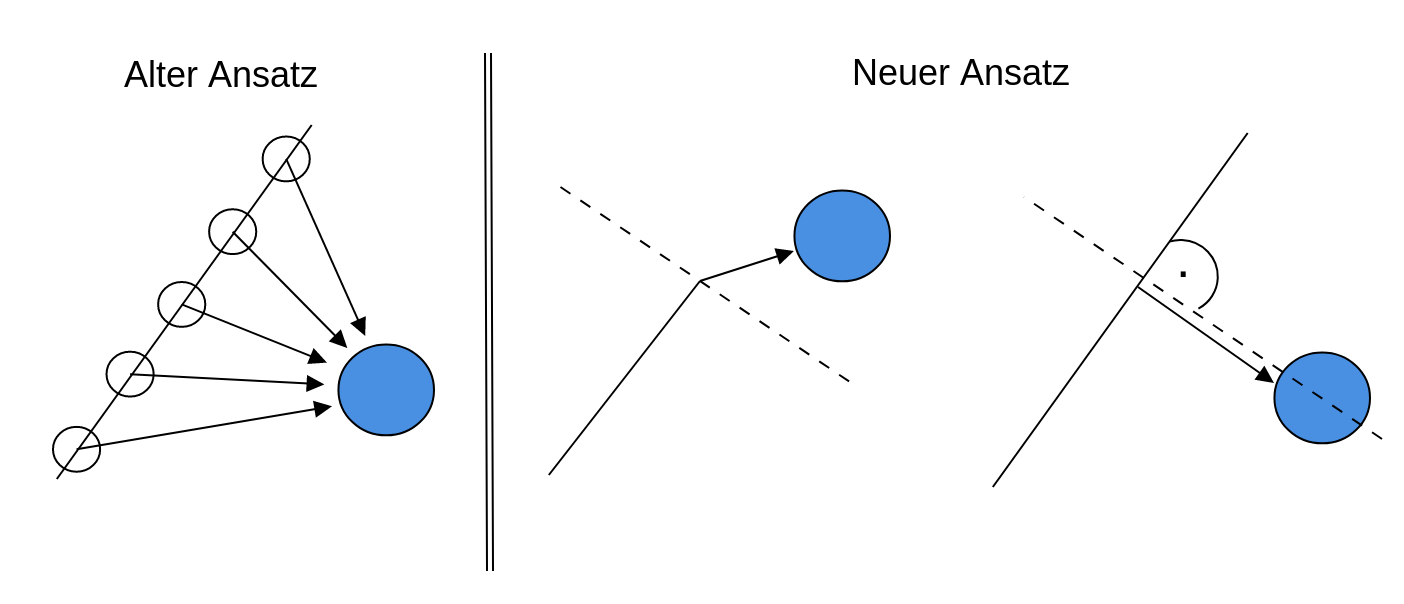
\includegraphics[width = 1.0\textwidth]{imgs/obstacle_force}
  \caption{Umsetzung der \emph{Obstacle Force}. Der alte Ansatz repräsentiert Hindernisse
  als viele Punkte, von denen der Fußgänger jeweils einzeln abgestoßen wird.
  Der neue Ansatz fällt ein Lot auf das Hindernis und stößt den Fußgänger orthogonal ab.
  Befindet sich der Fußgänger neben dem Hindernis, wird die Distanz zum nähergelegenen
  Endpunkt des Hindernisses herangezogen.}
  \label{fig:ObstacleForceOpt}
\end{figure}

Wie bereits angesprochen, ist die Umsetzung der Grid-Struktur sehr unflexibel und verhindert
einfachere Algorithmen mit Vektorgrafiken. Außerdem kann der LiDAR-Sensor aufgrund der
Rundungseffekte durch die Rasterisierung nicht hinreichend getestet werden, um die
Funktionstüchtigkeit der Sensorik sicherzustellen. Aus besagten Gründen wird die Repräsentation
von Hindernissen, Fußgängern, Fahrzeugen und Laserstrahlen auf einfache Vektorgrafiken umgestellt,
wie in Abschnitt \ref{sec:SimEnv} beschrieben. Dies hat zwar keine nennenswerten Auswirkungen auf das
Performance-Profil, aber ermöglicht eine Umstrukturierung und Vereinfachung der Simulationslogik.
Da \emph{RobotSF} nun im Vergleich zur ursprünglichen Simulationsumgebung von Caruso et. al
ungefähr 19-fach beschleunigt ist, können die Trainingsexperimente mit einer vertretretbaren
Wartezeit durchgeführt werden. Es werden noch einige kleinere Verbesserungen eingeführt,
um die Berechnung von Kollisionen und Kräften weit voneinander entfernter Entitäten
zu filtern. Dies soll in diesem Rahmen jedoch nicht weiter thematisiert werden.

\section{Mögliche Verbesserungen bezüglich Effizienz}
Wie der \emph{Mulit-Robot} Ansatz von Fan et. al \cite{fan2020distributed} demonstriert,
können gleichzeitig mehrere Fahrzeuge innerhalb derselben Simulationsumgebung trainieren,
sodass die Umgebung vektorisiert wird. Im Fall von \emph{RobotSF} würde dies zudem eine
Effizienzsteigerung bezüglich der Rechenzeit pro Simulationsschritt ermöglichen, da die
Berechnung der Kinematik und Sensorik pro Fahrzeug nur etwa 12\% Anteil am gesamten
Performance-Profil hat. Je nach Kartenmaterial kann in jeder Startzone je ein Fahrzeug
seine Route starten. Beispielsweise können Fahrzeuge auf dem Universitätscampus an 11
verschiedenen Orten starten, was die während des Trainings verwendeten 64
Simulationsumgebungen auf 6 reduziert. Im konkreten Fall ist in etwa eine 5-fache
Effizienzsteigerung möglich.

$$\eta = \left(\frac{0.88 \cdot 6 + 0.12 \cdot 64}{64}\right)^{-1} \approx 5$$

Durch eine Umstellung auf lokalitätsaffine Algorithmen im Zusammenspiel mit passenden
Datenstrukturen, z.B. Quad-Trees, wie es in der Grafikprogrammierung üblich ist,
sind weitere Effizienzsteigerungen bei der Umsetzung der Simulationsumgebung möglich.
Insbesondere kann die Dimensionierung des simulierten Kartenmaterials aufgrund der
lokalitätsaffinen Algorithmen nochmals deutlich vergrößert werden, sodass mehr
Startplätze und folglich auch weitere Fahrzeuge pro Umgebung denkbar sind.
Eine entsprechende Anpassung der Simulationsumgebung geht über den Umfang dieser Arbeit
deutlich hinaus, kann aber in Anbetracht der möglichen Verbesserungen durchaus
lohnenswert sein, zumal die Ergebnisse von Fan et. al \cite{fan2020distributed} ohnehin eine
Qualitätssteigerung der erlernten Fahrverhaltensweisen in Aussicht stellen.\\

Auch die Umsetzung des Trainingsalgorithmus mit Stable Baselines 3 hat noch
Verbesserungspotential. Während eines Trainingslaufs mit PPO werden ca. 30 Gigabyte
Arbeitsspeicher allokiert. Anhand der 64 parallel betriebenen Simulationen und einem
für das Sammeln der Trainingsdaten verwendeten Zeitintervall von 2048 Simulationsschritten
wären bei optimaler Speichernutzung aber nur ca. 450 Megabyte notwendig. Eine eigene
Implementierung von PPO mit TensorFlow 2 kann erfolgreich die Spiele Pong und CartPole
erlernen, ist jedoch nicht nennenswert effizienter. Um den Speicher adäquat kontrollieren
zu können, wäre eine Portierung hin zu einer hardwarenahen Sprache
sinnvoll. Um den Großteil der Simulationslogik behalten zu können, wird eine graduelle
Umstellung auf Mojo empfohlen. Neben der Unterstützung von eigenem Python Code sind
auch alle verwendeten Abhängigkeiten weiterhin verfügbar. Zusätzlich profitieren
in Mojo geschriebene Programme von einer Hyperparameteroptimierung der Cachegrößen.
Hierzu kompiliert Mojo zur Laufzeit mehrere Versionen des Codes und unterzieht diese
anschließend einigen Benchmarks, sodass eine optimale Performance mit der verwendeten
Maschine ohne tiefe Kenntnisse der Hardwareprogrammierung erzielt werden kann.

